\section{GUI}

\subsection{Klassendiagramm}

\begin{figure}[htbp] 
  \centering
  		 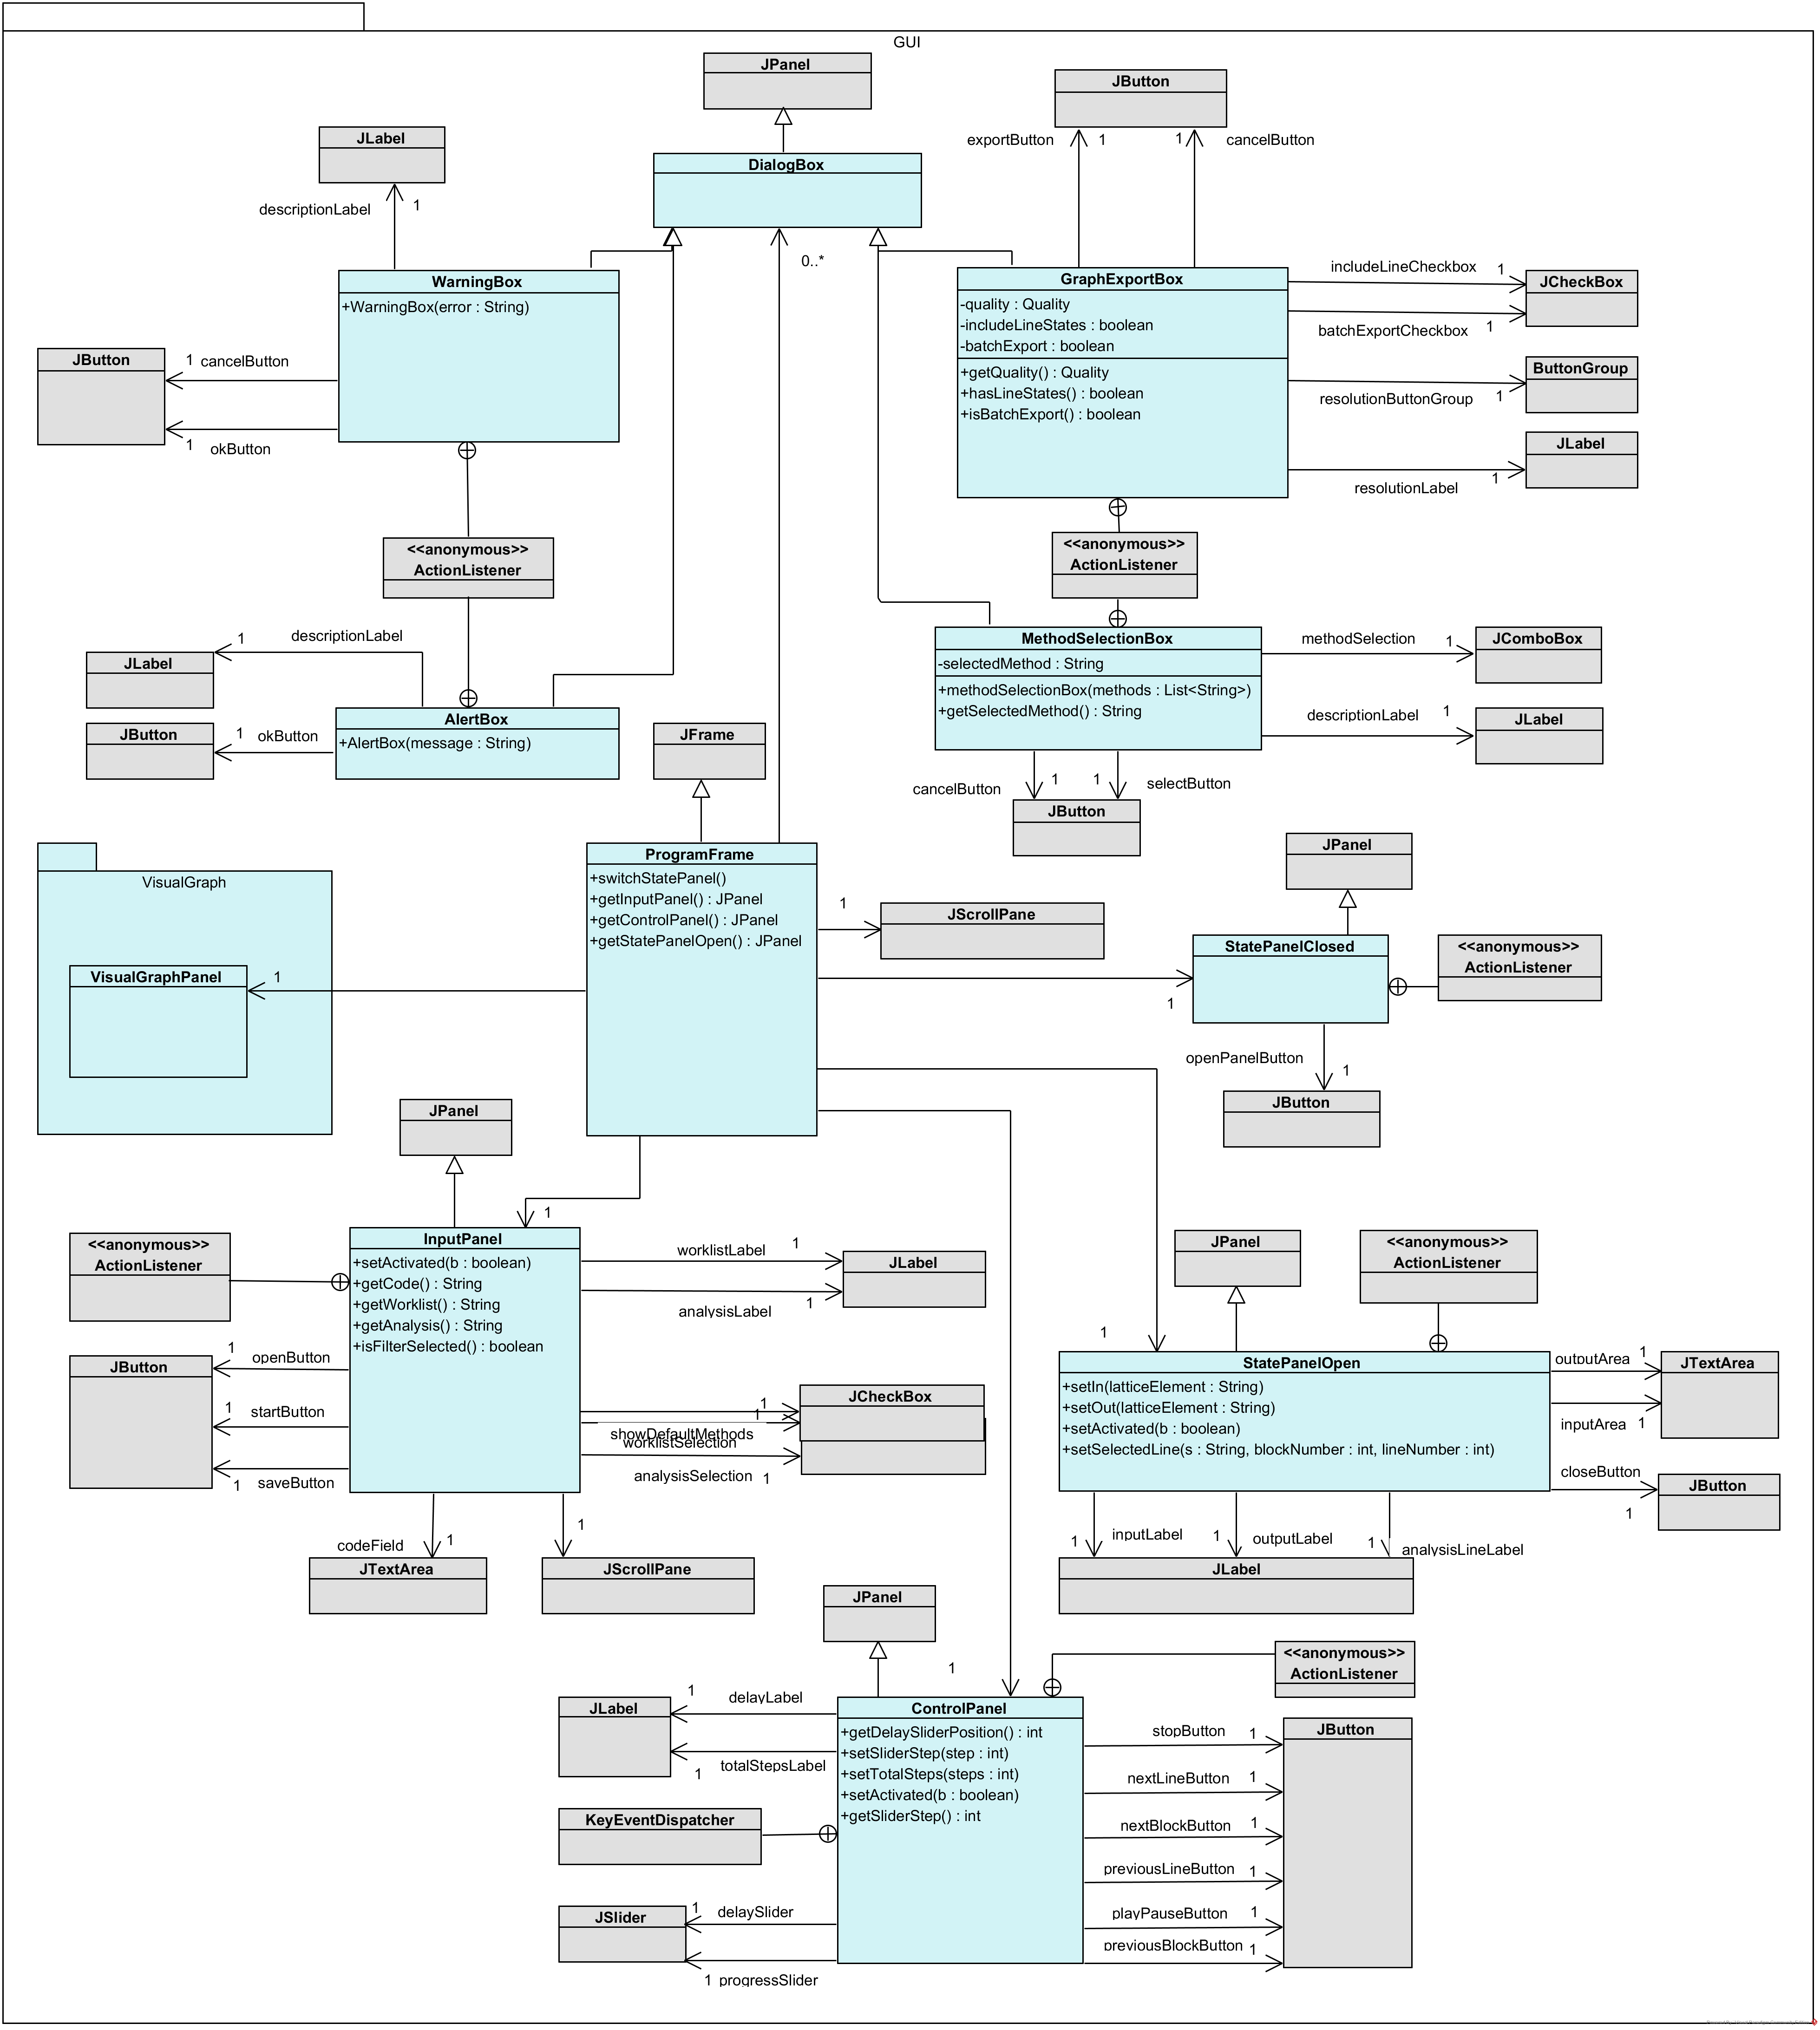
\includegraphics[width=1\textwidth]{Klassenuebersicht/GUI/GUI}
  \caption{Klassendiagramm des User Interfaces}
  \label{fig:UI}
\end{figure}

Das User Interface ist aus vier zentralen Panels aufgebaut. 
Das Input Panel stellt die für den Benutzer notwendige Funktion für das Einlesen von Code, das Auswählen der Analyse oder des Worklist-Algorithmus und das Starten der Analyse zur Verfügung. 
Über das ControlPanel kann der Benutzer die Animation seiner Analyse nachdem diese gestartet wurde kontrollieren. 
Die Änderungen, die sich dadurch am Graphen ergeben, werden im Graph Panel angezeigt. 
Dieses ist in ein eigenes Package ausgelagert (siehe Abschnitt x?????). 
Das StatePanel zeigt für jeden Analyseschritt die aktuellen/ausgewählten Bereich und den In- bzw. Out-Status des ausgewählten Bereichs an. 
Des Weiteren wird hier der Aufbau der verschiedenen DialogBoxes beschrieben.

\subsection{Klassenbeschreibung}

\subsubsection{ProgramFrame extends JFrame}

\textbf{Attribute}
\begin{itemize}
	\item private JPanel InputPanel
	\item private JPanel ControlPanel
	\item private JPanel StatePanelOpen
	\item private JPanel StatePanelClosed
	\item private JPanel VisualGraphPanel
\end{itemize}

\textbf{Konstruktor}\par
Standardkonstruktor.

\textbf{Methoden}
\begin{itemize}
	\item public void switchStatePanel()\par
	Macht entweder das StatePanelOpen, in dem die in und out Informationen gegeben werden sichtbar und blendet StatePanelClosed aus oder blendet StatePanelOpen aus und blendet StatePanelClosed ein. 
	\item public JPanel getInputPanel()\par
	Gibt das InputPanel zurück.
	\item public JPanel getControlPanel()\par
	Gibt das ControlPanel zurück.
	\item public JPanel getStatePanelOpen()\par
	Gibt das StatePanelOpen zurück.
\end{itemize}

\subsubsection{InputPanel extends JPanel}
\textbf{Attribute}
\begin{itemize}
	\item private JTextArea codeField
	\item private JButton startButton
	\item private JButton openButton
	\item private JButton saveButton
	\item private JLabel worklistLabel
	\item private JLabel analysisLabel
	\item private JCheckBox showDefaultMethods
	\item private JComboBox worklistSelection
	\item private JComboBox analysisSelection
\end{itemize}

\textbf{Konstruktor}\par
Standardkonstruktor.

\textbf{Methoden}
\begin{itemize}
	\item public void setActivated(boolean activ)\par
		Bestimmt, ob das InputPanel gerade verwendet werden kann oder nicht. Läuft eine aktuelle Analyse, ist das InputPanel deaktiviert und wird erst beim Abbruch der aktuellen Analyse wieder aktiv.
	\item public String getCode()\par
		Gibt den aktuell angezeigten Java-Code zurück.
	\item public String getWorklist()\par
		Gibt den Namen der aktuell ausgewählten Worklist zurück.
	\item public String getAnalysis()\par
		Gibt den Namen der aktuell ausgewählten Analyse zurück.
\end{itemize}

\subsubsection{ControlPanel extends JPanel}
\textbf{Attribute}
\begin{itemize}
	\item private JSlider delaySlider
	\item private JSlider progressSlider
	\item private JButton stopButton
	\item private JButton nextLineButton
	\item private JButton nextBlockButton
	\item private JButton previousLineButton
	\item private JButton previousBlockButton
	\item private JButton playPauseButton
	\item private JLabel totalStepsLabel
	\item private JLabel delayLabel
\end{itemize}

\textbf{Konstruktor}\par
Standardkonstruktor.

\textbf{Methoden}
\begin{itemize}
	\item public int getDelaySliderPosition()\par
		Gibt die Position des DelaySliders zurück.
	\item public void setSliderStep(int step)\par
		Setzt die Position des StepSliders an den genannten Schritt.
	\item public int getSliderStep()\par
		Gibt die Position des StepSliders zurück.
	\item public void setTotalSteps(int steps)\par
		Schreibt die Gesamtanzahl der Schritte, die die Analyse macht in das totalStepsLabel.
	\item public void setActivated(boolean activ)\par
		Bestimmt, ob das ControlPanel gerade verwendet werden kann oder nicht. Läuft eine aktuelle Analyse, ist das ControlPanel aktiviert und wird erst beim Abbruch der aktuellen Analyse 		
		wieder deaktiviert.
\end{itemize}

\subsubsection{StatePanelOpen extends JPanel}
\textbf{Attribute}
\begin{itemize}
	\item private JLabel analysisLineLabel
	\item private JLabel inputLabel
	\item private JLabel outputLabel
	\item private JTextArea inputArea
	\item private JTextArea outputArea
	\item private Jbutton closeButton
\end{itemize}

\textbf{Konstruktor}\par
Standardkonstruktor.

\textbf{Methoden}
\begin{itemize}
	\item public void setIn(String latticeElement)\par
		Setzt den In-Sate der aktuellen/ausgewählten Komponenten in die entsprechende JTextArea.
	\item public void setOut(String latticeElement)\par
		Setzt den Out-State der aktuellen/ausgewählten Komponente in die entsprechende JTextArea.
	\item public void setSelectedLine(String content, int blockNumber, int lineNumber)\par
		Setzt den Inhalt der ausgewählten Komponente in die entsprechende JTextArea und fügt die Nummer des Blockes oder der Zeile hinzu.
	\item public void setActivated(boolean activ)\par
		Bestimmt, ob das StatePanelOpen gerade verwendet werden kann oder nicht. Läuft eine aktuelle	Analyse, ist das StatePanelOpen aktiviert und wird erst beim Abbruch der aktuellen Analyse wieder deaktiviert.
\end{itemize}

\subsubsection{StatePanelClose extends JPanel}
\textbf{Attribute}
\begin{itemize}
	\item private JButton openPanelButton
\end{itemize}

\textbf{Konstruktor}\par
Standardkonstruktor.

\textbf{Methoden}
\begin{itemize}
	\item Keine benötigten öffentlichen Methoden
\end{itemize}

\subsubsection{DialogBox extends JPanel}
\textbf{Attribute}
\begin{itemize}
 	\item Keine benötigten öffentlichen Attribute
\end{itemize}

\textbf{Konstruktor}\par
Standardkonstruktor

\textbf{Methoden}
\begin{itemize}
	\item Keine benötigten öffentlichen Methoden
\end{itemize}

\subsubsection{MethodSelectionBox extends DialogBox}
\textbf{Attribute}
\begin{itemize}
	\item private String selectedMethod
	\item private JCombobox methodSelection
	\item private JLabel despriptionLabel
	\item private JButton cancelButton
	\item private JButton selectButton
\end{itemize}

\textbf{Konstruktor}\par
Standardkonstruktor.

\textbf{Methoden}
\begin{itemize}
	\item public void methodSelectionBox(List<String> methods)\par
		Übergibt eine Liste von im Code vorhandenen Methoden, die in der JComboBox angezeigt werden sollen.
	\item public String getSelectedMethod()\par
		Gibt zurück, welche Methode aktuell ausgewählt ist.
\end{itemize}


\subsubsection{GraphExportBox extends DialogBox}
\textbf{Attribute}
\begin{itemize}
	\item private Quality quality
	\item private boolean includeLineSTates
	\item private boolean batchExport
	\item private JCheckBox batchExportCheckbox
	\item private JCheckBox includeLineCheckbox
	\item private ButtonGroup resolutionButtonGroup
	\item private JButton exportButton
	\item private JButton cancelButton
	\item private JLabel resolutionLabel
\end{itemize}

\textbf{Konstruktor}\par
Standardkonstruktor.

\textbf{Methoden}
\begin{itemize}
	\item public Quality getQuality()\par
		Gibt die ausgewählte Qualität zurück.
	\item public boolean hasLineStates()\par
		Gibt zurück, ob die In- und Out-States der Zeilen mit in das Bild aufgenommen werden sollen.
	\item public boolean isBatchExport()\par
		Gibt zurück, ob BatchExport ausgewählt wurde.
\end{itemize}


\subsubsection{WarningBox extends DialogBox}
\textbf{Attribute}
\begin{itemize}
	\item private JLabel descriptionLabel
	\item private JButton cancelButton
	\item private JButton okButton
\end{itemize}

\textbf{Konstruktor}
\begin{itemize}
	\item public void WarningBox(String error)
	Schreibt die entsprechende Nachricht in das Label.
\end{itemize}

\textbf{Methoden}
\begin{itemize}
	\item Keine benötigten Methoden.
\end{itemize}

\subsubsection{AlertBox extends DialogBox}
\textbf{Attribute}
\begin{itemize}
	\item private JLabel descriptionLabel
	\item private JButton okButton
\end{itemize}

\textbf{Konstruktor}
\begin{itemize}
	\item public void AlertBox(String message)\par
	Schreibt die entsprechende Nachricht in das Label.
\end{itemize}

\textbf{Methoden}
\begin{itemize}
	\item Keine benötigten Methoden
\end{itemize}


